%!TEX TS-program = pdflatex
%!TEX encoding = UTF-8 Unicode


\chapter{Parallel Processing with GPUs}% (fold)
\label{cha:parallel_processing_with_gpu} 

In recent years more and more parallel hardware appeared on the computing market
with different architecture specialised for different problems. One of the recent
and most discussed architectures is the \gls{GPU}. The major player in the field
are  \gls{ATI} and the \slcsmallcaps{NVIDIA} corporation that both offer 
\glspl{SDK} and \glspl{GPU} for general purpose computing. Beside \glspl{GPU} there
are a lot other companies that offer parallel hardware architectures listed in 
\autoref{ch:literature_review}. Following a brief introduction to parallel
 architectures important to specify and identify the sort of parallelism offered
by \glspl{GPU} and other hardware.

\section{Parallel Architectures}
\label{sec:parallel_architectures} 

There are several ways how operations in a system can be executed in parallel. 
\begin{itemize}
	\item \gls{SISD} This is the common von Neumann model, which is a system which
	exploits no parallelism.
	\item \gls{SIMD} operations inside a functional unit where one operation is 
	simultaneously applied to a vector of 2--16 components. Many modern \glspl{CPU}
	have now \gls{SIMD} units but every manufacturer is naming them differently
(e.g. Altivec, \gls{VMX}, \gls{MMX}, \gls{SSE}).
	\item \gls{MIMD} threads, cores, processors each executing on its own data. Many
	parallel architectures can be mapped onto the \gls{MIMD} architecture. 
	
	There is as well the \gls{MISD} classification which is a uncommon architecture but
	can be used e.g. in fault-tolerance systems where different units generate a result 
	on the same data and they must all agree on the result. For common parallel architectures
	its not used. By far the most used classification for parallel systems is \gls{MIMD}
	that can be further divided into two more classifications. 
	
	\item \gls{SPMD} threads within a core where one program is running on the core
	and different threads are executing with different data. A combination of the 
	\gls{SIMD} and \gls{SPMD} model is used on modern \glspl{GPU}.
	\item \gls{MPMD} threads executing a different program on different data. The 
	\gls{MPMD} threads reside either within a single core (hardware threads,
	hyper-threading) or in distinct cores of a processor or lastly in different
	processors.
\end{itemize}
The above classification is based upon the number of concurrent instruction and 
data streams available in a system. The classification comes from \citeauthor{citeulike:3789408}
in \citep{citeulike:3789408}. Today there is  still no satisfactory characterisation 
of the different types of parallel systems. Flynn's taxonomy was a first step, 
today there are much more characterisations that refine the previous mentioned. 

To characterise the \gls{GPU} one needs two classifications. First of all in
each \gls{GPU} there are threads that are grouped together which are executing 
one instruction on different data. These \gls{SIMD} groups are further grouped
to a \gls{SPMD} system where all of these, there can be many of them, are
executing the same program. On the basis of \glspl{NVIDIA} Tesla architecture 
a more detailed look at a \gls{GPU} will be given in the next sections.


\section{The Tesla Architecture}% (fold)
\label{sub:the_tesla_architecture} 
The Tesla architecture announced 2007 and developed by \gls{NVIDIA} is the first
\gls{GPU} highly specialised for raster operations and more important
for general purpose computing. Formerly \glspl{GPU} had fixed-function
pipelines and separate processing units with no ability for programmability to
the vertex and fragment stages of the pipeline. In recent years manufacturers of
\glspl{GPU} added more and more programmability to the different stages
of the pipeline and at the same time general purpose computing capabilities
\citep{citeulike:3844545}. Furthermore manufacturers introduced the  \gls{USM} 
that unifies the processing units allowing for better
utilisation of  \gls{GPU} resources. The resources needed by different
shaders varies greatly and the unified design can overcome this issue by
balancing the load among vertex, fragment and geometry functionality
\citep{citeulike:3145468}.

\begin{figure}[ht]
\centering
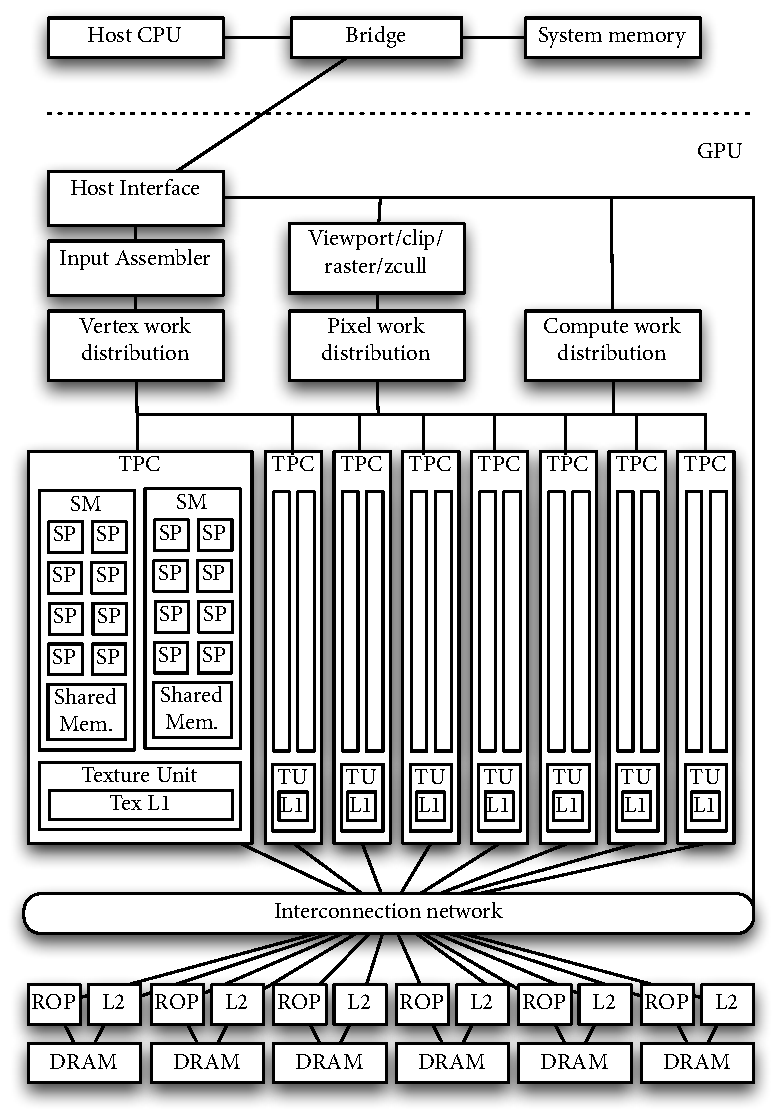
\includegraphics[width=4in]{gfx/tesla_architecture} 
\caption{Tesla Architecture} 
\label{fig:tesla_architecture} 
\end{figure} 

The \autoref{fig:tesla_architecture} shows the Tesla architectures. As mentioned
above the new \gls{GPU} architectures are a radical departure from traditional
\gls{GPU} design. The Tesla 8 Series has 16 multiprocessors. Each multiprocessor
is composed of 8 streaming processors, 128 processors in total. Each streaming
multiprocessor has 16 \gls{KB} of shared memory a L1 cache attached and has access
to a texture unit. A streaming processor consists of a scalar \gls{ALU} and
performs floating point operations. 32 streaming processor build up a \gls{SIMD}
unit in {\slcsmallcaps{NVIDIA}} terms called warp, in that one instruction is executed. The Tesla
C870 has 1.5 \gls{GB} \gls{GDDR3} graphics memory, 519 \glspl{GFLOP} of peak
performance and \unitfrac[77]{\gls{GB}}{s} peak memory bandwidth. Many massively
data-parallel algorithms can be run sufficiently on this specialised
architecture \citep{citeulike:3145468}. Programming for this architecture is
done with \gls{CUDA} the C language extension which will be covered in the next
section.


\paragraph{The Mainstream GPU} % (fold)
\label{par:the_mainstream_gpu}
There are two solutions for \gls{GPU} computing from {\slcsmallcaps{NVIDIA}}. Firstly the
\emph{Tesla 8 Series} which is specifically designed for high-performance
computing. The \emph{Tesla 8 Series} is available as an \gls{PCIE} add-in card,
desk-side computing system and as a \gls{1U} computing system. All this systems have
no display port and hence they can exclusively be used as a computing nodes. 

The second solution are the mainstream \emph{GeForce 8 Series} card that
is mainly used for gaming. The architecture of these both solutions is the same
(\gls{USM}) they differentiate only in the magnitude of some performance
characteristics (memory size, peak memory bandwidth, peak \gls{GFLOP}). The
advantage of a mainstream \gls{GPU} is that the visualisation can be done on the
same card and the low price. 

For the purpose of this thesis a \emph{GeForce 8800 GTS 512} card will be
used. The main performance characteristics are shown in
\autoref{tab:tesla_geforce_mem} and \autoref{tab:tesla_geforce}. For reference
the \emph{Tesla C870} card is shown as well.

\begin{table}[ht]
	\centering
	%\pgfkeys{/pgf/number format/.cd,fixed zerofill,precision=2}
	\pgfplotstabletypeset[
%		column type=r,
		columns={Card, {Memory Size}, {Bandwidth}, Clock},
		columns/Card/.style={string type},
		columns/{Memory Size}/.style={column name={Memory Size [\protect\slcsmallcaps{MB}]}},
		columns/{Bandwidth}/.style={column name={Bandwidth [\unitfrac{GB}{s}]}},
		columns/{Clock}/.style={column name={Clock [\slcsmallcaps{MHz}]}},
	]{Tables/tesla.geforce.memory.data}
  	\caption{Memory performance characteristics for Tesla and GeForce}
  	\label{tab:tesla_geforce_mem}
\end{table}

The most significant difference between the two cards is the peak bandwidth. There
are several algorithms which rely on a high bandwidth which would increase the
run time on as \emph{8800 GTS} card even if it has a higher peak floating
point operations per second as seen in  \autoref{tab:tesla_geforce}. 

\begin{table}[ht]
	\centering
%	\pgfkeys{/pgf/number format/.cd,fixed zerofill,precision=2}
	\pgfplotstabletypeset[
%		column type=r,
		columns={Card, {No. of Stream Processors}, GFlops, Clock},
		columns/{GFlops}/.style={column name={\slcsmallcaps{GFlops}}},
		columns/{Clock}/.style={column name={Clock [\slcsmallcaps{MHz}]}},
		columns/Card/.style={string type}
	]{Tables/tesla.geforce.data}
  	\caption{Computing performance characteristics for Tesla and GeForce}
  	\label{tab:tesla_geforce}
\end{table}

Every card of the \emph{GeForce 8 Series} can be programmed with \gls{CUDA} an
\gls{API} for \gls{GPU} computing. What \gls{CUDA} is and how to use it will 
be explained in the next section. 
% section the_tesla_architecture (end)


\section{Common Unified Device Architecture (CUDA)}% (fold)
\label{sub:common_unified_device_architecture_cuda_} 
In 2007, {\slcsmallcaps{NVIDIA}} introduced an extended \gls{ANSI} C programming model and
software environment the compute unified device architecture. The reason why
\gls{CUDA} was born is that parallelism is increasing rapidly with Moore's law
\footnote{Processor count is doubling every 18 - 24 months} and the challenge is
to develop parallel application software that scales transparently with the
number of processor cores. The main goals when \gls{CUDA} was developed were
that it scales to hundreds of cores, thousands of parallel threads and it allows
heterogeneous computing (\gls{CPU} + \gls{GPU}). All this considerations led to
the result that \gls{CUDA} runs on any number of processors without recompiling
an the parallelism applies to both \glspl{CPU} and \glspl{GPU} 
\citep{citeulike:3839013}.

\Gls{CUDA} is C with minimal extensions and defines a programming and memory model.
There are three key abstractions in \gls{CUDA}, a hierarchy of thread groups, shared
memories and barrier synchronisation \citep{citeulike:3325943} that are exposed
to the developer. \Gls{CUDA} uses extensive multithreading where threads express
fine-grained instruction, data and thread parallelism that are grouped into
thread blocks which express coarse grained data and task parallelism. The
developer has to rethink about his algorithms to be aggressively parallel.
The problem has to be split into independent coarse sub-problems and at finer
level into fine-grained sub-problems that can be solved cooperatively
\citep{citeulike:3325943}.

\Gls{CUDA} has been accepted be many developers which can be seen by the huge
amount of already developed software and contributions to the \gls{CUDA}
zone \footnote{http://www.nvidia.com/cuda}.

A brief look shows the \gls{CUDA} computing sweet 
spots\citep{citeulike:3839013}

\begin{itemize}
	\item High arithmetic intensity (Dense linear algebra, PDEs, n-body, 
			finite difference, \ldots) 
	\item High bandwidth (Sorting, database,  sequencing, virus scanning, genomics, \ldots) 
	\item Visual computing: (Graphics, image processing, tomography, 
			machine vision, \ldots) 
	\item Computational modelling, science, engineering, finance, ... 			
\end{itemize} 

This is just a small snapshot of algorithms that can be used with \gls{CUDA} on
\glspl{GPU}. For a more extensive list and speedups compared to high-end
\glspl{CPU} see the webpage of {\slcsmallcaps{NVIDIA}}
\href{http://www.nvidia.com/cuda}{\gls{CUDA} zone}. 
% section_unified_device_architecture_cuda_ (end)

\section{CUDA Programming Model}% (fold)
\label{sub:cuda_programming_model} 
The \gls{CUDA} programming model exposes the graphics processor as a highly
multithreaded coprocessor. The \gls{GPU} is viewed as a compute device to the
host that has its own device memory and runs many threads in parallel.

Applications are accelerated by executing data parallel portions of the
algorithm on the \gls{GPU} as \emph{kernels} which run in parallel on many
threads. There are some major differences between \gls{CPU} and
\gls{GPU} threads. A \gls{GPU} needs thousands of threads for full efficiency
where \glspl{CPU} only need a few of them. \Gls{GPU} threads have a very little
creation overhead and are extremely lightweight compared to \gls{CPU} threads.

\paragraph{Thread Batching}% (fold)
\label{par:thread_batching} 
A kernel is executed as a grid of thread blocks where data memory space is
shared by all threads. A thread block is a batch of threads that can cooperate
with each other by synchronising there execution\footnote{For hazard free shared
memory access} and efficiently share data through the low latency shared
memory. Two threads from two different blocks can cooperate with atomic 
functions through the global memory. The identification of a thread is 
accomplished through block and thread ids which are assigned to each thread at 
creation time. 
% paragraph thread_batching (end)

\paragraph{Block and Thread IDs}% (fold)
\label{par:block_and_thread_ids} 
Every thread and block has a unique id. As a result of this each thread can
decide what data to work on. For every block there is a assigned id in \gls{1D}
or \gls{2D} layout. Thread ids can be accessed either with \gls{1D}, \gls{2D} or
\gls{3D} coordinates similar to multidimensional arrays. It simplifies memory
addressing when processing multidimensional data( e.g image processing, matrix
multiplication or solving partial differential equations on volumes). The data
can reside in several levels of the device memory. % paragraph
%block_and_thread_ids (end)

\paragraph{Device Memory Space}% (fold)
\label{par:device_memory_space} 
The memory space is a hierarchy of several memory types that can be accessed per
thread, block, grid and the host. The threads have access to all memory levels
beginning with the \gls{RW} registers, local, shared, global, \gls{RO}
texture and constant memory. The grids have only access to global, constant
and texture memory. Whereas the \gls{CPU} can \gls{RW} global, constant and texture
memories.

Global, constant and texture memory have long latency accesses. They reside
off-chip where registers local\footnote{Not true for older \glspl{GPU} chips
where local data is spilled out to global memory} and shared memory resides
on-chip. The global, constant and texture memory are mainly used for
communication of \gls{RW} data between host and device where the contents is
visible to all threads. As mentioned above texture and constant memory can be
written by the host where constants and data are initialised.
% paragraph device_memory_space (end)


\section{A Simple Example}% (fold)
\label{sub:a_simple_example} 
This simple example will show the structure of an \gls{CUDA} program. The executing
kernel will do some easy calculations on the data provided, load the data into
shared memory  and write back the results to the global memory. 

A \gls{CUDA} program has a specific structure where the major parts are
described in this paragraph. The first thing to do is to initialise the device
and some auxiliary variables. The \autoref{lst:init} shows the
initialisation.

%
\begin{lstlisting}[caption=Hardware initialisation, label=lst:init]
CUT_DEVICE_INIT(argc, argv);

uint32_t num_threads = 32;
uint32_t mem_size = sizeof(float) * num_threads;				
\end{lstlisting} 
%

Since the \gls{GPU} is attached to the \gls{PCIE} bus the host has no direct
access to the global, constant and texture memory and has to transfer the data
back and forth with the \gls{DMA} engine of the device. This is accomplished
through the \gls{CUDA} \gls{API} calls that initiate the transfer. Before any
transfer can be done one has to allocate memory on the host and on the device
for input and output data. This is shown in listing \autoref{lst:datatransfer}.


\begin{lstlisting}[caption=Data transfer of data, label=lst:datatransfer]
// allocate host memory 
float* h_idata = (float*) malloc(mem_size);
// allocate device memory 
float* d_idata; cudaMalloc((void**) &d_idata, mem_size);
// allocate device memory for result
float* d_odata; cudaMalloc((void**) &d_odata, mem_size);
// allocate mem for the result on host side
float* h_odata = (float*) malloc( mem_size);
// copy host memory to device 
cudaMemcpy(d_idata, h_idata, mem_size, cudaMemcpyHostToDevice);
\end{lstlisting} 


After setting up the input data the setup execution parameters are defined that
are used to startup the kernel. The \textsf{grid(1, 1, 1)} statement defines
a multi-dimensional array of grids $x=1, y=1, z=1$ whereas the
\textsf{threads(num\_threads, 1, 1)} defines a multi-dimensional array of
threads $x=num\_threads, y=1, z=1$ which are actually \gls{1D} arrays.
\autoref{lst:execution} shows the call of the kernel with its input and
output data.


\begin{lstlisting}[caption=Execution of the Kernel, label=lst:execution]
// setup execution parameters
dim3  grid( 1, 1, 1);
dim3  threads(num_threads, 1, 1);

// execute the kernel
kernel<<< grid, threads, mem_size >>>(d_idata, d_odata);
\end{lstlisting} 

Attention must be paid to the both statements that define the array for the grid
and the thread block. The size of the array or the amount of threads dependent
on three factors, (1) register usage, (2) shared and (3) local memory usage per
thread. Accumulated per grid they are not allowed to pass a certain size.
Calculations how the existing resources are used can easily be calculated with
the \emph{CUDA occupancy calculator}. The performance of the application depends
on how good/bad the existing resources are exploited.

If everything went well the host can copy the data from device memory
to host memory and check, visualise or store the calculated values.
\autoref{lst:result} shows the last steps before exiting the program.

\begin{lstlisting}[caption=Retrieving of the Results, label=lst:result]
// check if kernel execution generated and error
CUT_CHECK_ERROR("Kernel execution failed");
 
// copy result from device to host
cudaMemcpy(h_odata, d_odata, sizeof( float) * num_threads, 
           cudaMemcpyDeviceToHost);

// cleanup memory free(x), free(y), free(z) ...
CUT_EXIT(argc, argv);
\end{lstlisting} 

The previous listings showed the host code and how to launch a kernel on the
device. The \autoref{lst:device} shows the device code portion. There are
several qualifiers that define which function is compiled for which processing
unit. The \textsf{\_\_global\_\_} qualifier specifies that this function is run
on the device and hence compiled for the \gls{GPU} where the
\textsf{\_\_host\_\_} qualifier specifies that this function is only run on the
host and not on the device. There are more function specifiers that can be
looked up in \citep{citeulike:3325943}.

For data there are as well qualifiers where one can specify where the data is
located, either in constant, global or shared memory. In \autoref{lst:device}
the \textsf{\_\_shared\_\_} qualifier is used. The device will use the shared
memory to preload the data for faster access.

\begin{lstlisting}[caption=CUDA device code, label=lst:device]
#include <stdio.h>

#define SDATA(index) CUT_BANK_CHECKER(sdata, index)
// Simple test kernel for device functionality
__global__ void kernel( float* g_idata, float* g_odata) 
{
  // shared memory, the size is determined by the host application
  extern  __shared__  float sdata[];

  // access thread id 
  const unsigned int tid = threadIdx.x;
  // access number of threads in this block 
  const unsigned int num_threads = blockDim.x;

  // read in input data from global memory
  // use the bank checker macro to check for bank conflicts
 	// during host emulation 
  SDATA(tid) = g_idata[tid];
  __syncthreads();

  // perform some computations 
  SDATA(tid) = (float) num_threads * SDATA( tid);
  __syncthreads();

  // write data to global memory 
  g_odata[tid] = SDATA(tid);
} 
\end{lstlisting} 


After loading the data the kernel just multiplies the thread-id with the number
of threads and saves the result back to global memory where the host can pick up
the result.
% section a_simple_example (end)
% section cuda_programming_model (end)
% section background_to_the_project (end)

\section{Porting Strategy for GPUs}% (fold)
\label{sec:porting_strategies_for_gpu} 
This section  is a high-level overview of the porting process to not only
the \gls{GPU} it can be rather seen as general porting process to parallel 
hardware. It includes strategies that help through the porting process. It 
breaks down the porting process into a series of discrete steps. 

The steps included here are not the only path through the porting process because
the porting process is flexible and has to be adapted slightly for every hardware. 

In general, one will follow these steps when porting an algorithm to the \gls{GPU}
\begin{itemize}
	\item Algorithm complexity study. Profile the code, find the most compute
intensive parts analyse the parts of the algorithm which could be parallelised.
	\item Data layout/locality and Data flow analysis. Look for independent task or 
	independent data to exploit task or data parallelism.
	\item Experimental partitioning and mapping of the algorithm and program 
		structure to the architecture. 
	\item Develop \gls{CPU} control, \gls{CPU} scalar/multicore code
	\item Develop \gls{CPU} control, partitioned \gls{GPU} scalar code (Communication, 
		synchronisation, latency handling)
	\item Transform \gls{GPU} scalar code to \gls{GPU}threaded code, multi \gls{GPU} code. 
	Exploit all available cores and devices on the system. 
	\item Re-balance the computation / data movement. 
	\item Other optimisation considerations (load balancing, bottlenecks...)
\end{itemize}
% subsubsection typical_software_development_flow (end)


